% This is the Reed College LaTeX thesis template. Most of the work
% for the document class was done by Sam Noble (SN), as well as this
% template. Later comments etc. by Ben Salzberg (BTS). Additional
% restructuring and APA support by Jess Youngberg (JY).
% Your comments and suggestions are more than welcome; please email
% them to cus@reed.edu
%
% See http://web.reed.edu/cis/help/latex.html for help. There are a
% great bunch of help pages there, with notes on
% getting started, bibtex, etc. Go there and read it if you're not
% already familiar with LaTeX.
%
% Any line that starts with a percent symbol is a comment.
% They won't show up in the document, and are useful for notes
% to yourself and explaining commands.
% Commenting also removes a line from the document;
% very handy for troubleshooting problems. -BTS

% As far as I know, this follows the requirements laid out in
% the 2002-2003 Senior Handbook. Ask a librarian to check the
% document before binding. -SN

%%
%% Preamble
%%
% \documentclass{<something>} must begin each LaTeX document
\documentclass[12pt,twoside]{reedthesis}
% Packages are extensions to the basic LaTeX functions. Whatever you
% want to typeset, there is probably a package out there for it.
% Chemistry (chemtex), screenplays, you name it.
% Check out CTAN to see: http://www.ctan.org/
%%
\usepackage{graphicx,latexsym}
\usepackage{amsmath}
\usepackage{amssymb,amsthm}
\usepackage{longtable,booktabs,setspace}
\usepackage{chemarr} %% Useful for one reaction arrow, useless if you're not a chem major
\usepackage[hyphens]{url}
% Added by CII
\usepackage{hyperref}
\usepackage{lmodern}
% End of CII addition
\usepackage{rotating}

% Next line commented out by CII
%%% \usepackage{natbib}
% Comment out the natbib line above and uncomment the following two lines to use the new 
% biblatex-chicago style, for Chicago A. Also make some changes at the end where the 
% bibliography is included. 
%\usepackage{biblatex-chicago}
%\bibliography{thesis}


% Added by CII (Thanks, Hadley!)
% Use ref for internal links
\renewcommand{\hyperref}[2][???]{\autoref{#1}}
\def\chapterautorefname{Chapter}
\def\sectionautorefname{Section}
\def\subsectionautorefname{Subsection}
% End of CII addition

% Added by CII 
\usepackage{caption}
\captionsetup{width=5in}
% End of CII addition

% \usepackage{times} % other fonts are available like times, bookman, charter, palatino


% To pass between YAML and LaTeX the dollar signs are added by CII
\title{My Final College Paper}
\author{Your R. Name}
% The month and year that you submit your FINAL draft TO THE LIBRARY (May or December)
\date{May 20xx}
\division{Mathematics and Natural Sciences}
\advisor{Advisor F. Name}
%If you have two advisors for some reason, you can use the following
% Uncommented out by CII
% End of CII addition

%%% Remember to use the correct department!
\department{Mathematics}
% if you're writing a thesis in an interdisciplinary major,
% uncomment the line below and change the text as appropriate.
% check the Senior Handbook if unsure.
%\thedivisionof{The Established Interdisciplinary Committee for}
% if you want the approval page to say "Approved for the Committee",
% uncomment the next line
%\approvedforthe{Committee}

% Added by CII
%%% Copied from knitr
%% maxwidth is the original width if it's less than linewidth
%% otherwise use linewidth (to make sure the graphics do not exceed the margin)
\makeatletter
\def\maxwidth{ %
  \ifdim\Gin@nat@width>\linewidth
    \linewidth
  \else
    \Gin@nat@width
  \fi
}
\makeatother

\renewcommand{\contentsname}{Table of Contents}
% End of CII addition

\setlength{\parskip}{0pt}

% Added by CII

\providecommand{\tightlist}{%
  \setlength{\itemsep}{0pt}\setlength{\parskip}{0pt}}

\Acknowledgements{
I want to thank a few people.
}

\Dedication{
You can have a dedication here if you wish.
}

\Preface{
This is an example of a thesis setup to use the reed thesis document
class.
}

\Abstract{
The preface pretty much says it all. \par  Second paragraph of abstract
starts here.
}

% End of CII addition
%%
%% End Preamble
%%
%

\begin{document}

% Everything below added by CII
      \maketitle
  
  \frontmatter % this stuff will be roman-numbered
  \pagestyle{empty} % this removes page numbers from the frontmatter

      \begin{acknowledgements}
      I want to thank a few people.
    \end{acknowledgements}
  
      \begin{preface}
      This is an example of a thesis setup to use the reed thesis document
      class.
    \end{preface}
  
      \hypersetup{linkcolor=black}
    \setcounter{tocdepth}{2}
    \tableofcontents
  
      \listoftables
  
      \listoffigures
  
      \begin{abstract}
      The preface pretty much says it all. \par  Second paragraph of abstract
      starts here.
    \end{abstract}
  
      \begin{dedication}
      You can have a dedication here if you wish.
    \end{dedication}
  
  \mainmatter % here the regular arabic numbering starts
  \pagestyle{fancyplain} % turns page numbering back on

  \chapter*{Introduction}\label{introduction}
  \addcontentsline{toc}{chapter}{Introduction}
  
  Welcome to the \emph{R Markdown} thesis template. This template is based
  on (and in many places copied directly from) the \LaTeX~template, but
  hopefully it will provide a nicer interface for those that have never
  used \TeX~or \LaTeX~before. Using \emph{R Markdown} will also allow you
  to easily keep track of your analyses in \textbf{R} chunks of code, with
  the resulting plots and output included as well. The hope is this
  \emph{R Markdown} template gets you in the habit of doing reproducible
  research, which benefits you long-term as a researcher, but also will
  greatly help anyone that is trying to reproduce or build onto your
  results down the road.
  
  Hopefully, you won't have much of a learning period to go through and
  you will reap the benefits of a nicely formatted thesis. The use of
  \LaTeX~in combination with \emph{Markdown} is more consistent than the
  output of a word processor, much less prone to corruption or crashing,
  and the resulting file is smaller than a Word file. While you may have
  never had problems using Word in the past, your thesis is likely going
  to be about twice as large and complex as anything you've written
  before, taxing Word's capabilities. After working with \emph{Markdown}
  and \textbf{R} together for a few weeks, we are confident this will be
  your reporting style of choice going forward.
  
  \subsubsection{Why use it?}\label{why-use-it}
  
  \emph{R Markdown} creates a simple and straightforward way to interface
  with the beauty of \LaTeX. Packages have been written in \textbf{R} to
  work directly with \LaTeX~to produce nicely formatting tables and
  paragraphs. In addition to creating a user friendly interface to \LaTeX,
  \emph{R Markdown} also allows you to read in your data, to analyze it
  and to visualize it using \textbf{R} functions, and also to provide the
  documentation and commentary on the results of your project. Further, it
  allows for \textbf{R} results to be passed inline to the commentary of
  your results. You'll see more on this later.
  
  \subsubsection{Who should use it?}\label{who-should-use-it}
  
  Anyone who needs to use data analysis, math, tables, a lot of figures,
  complex cross-references, or who just cares about the final appearance
  of their document should use \emph{R Markdown}. Of particular use should
  be anyone in the sciences, but the user-friendly nature of
  \emph{Markdown} and its ability to keep track of and easily include
  figures, automatically generate a table of contents, index, references,
  table of figures, etc. should make it of great benefit to nearly anyone
  writing a thesis project.
  
  \chapter{Chapter 1}\label{chapter-1}
  
  \section{1.1 Trees and Random Forests}\label{trees-and-random-forests}
  
  \subsection{Trees}\label{trees}
  
  Decision trees may be familiar to many with a background in the social
  or medical sciences as convenient ways to represent data and can assist
  in decision making. Morgan and Sonquist (1963) derived a way for
  constructing trees motivated by the specific feature space of data
  collected from interviews and surveys. Unlike, say agricultural data
  which involves mostly numerical variables like rainfall, the data
  collected from interviews is mostly categorical. On top of this issue,
  the datasets Morgan and Sonquist dealt with had few participants (n) and
  much data collected on them (p). To continue with their list of
  difficulties, there was reason to believe that there were lurking errors
  in the variables that would be hard identify and quantify. Lastly, many
  of the predictors were correlated and Morgan and Sonquist doubted that
  the additive assumptions of many models would be appropriate for this
  data. Morgan and Sonquist noted that while many statistical methods
  would have a difficult time accurately parsing this data, a clever
  researcher with quite a lot of time could create a suitable model simply
  by grouping values in the feature space and predicting that the response
  corresponding to these values would be the mean of the observed
  responses given the grouped conditions. Their formalization of this
  procedure in terms of ``decision rules'' laid the ground work for future
  research on decision trees.
  
  In 1984, Breiman et al introduces a revolutionary new algorithm for
  trees. \textbf{Need to acquire} \emph{Classification and Regression
  Trees} \textbf{to make sure the method discused in MASS is the same that
  Breiman uses/is used in} \texttt{randomForest}
  
  \textbf{Tree Algorithm} CART?
  
  Begin by considering the entire feature space \(X_1, ..., X_n\). Then:
  
  \begin{enumerate}
  \def\labelenumi{\arabic{enumi}.}
  \item
    Consider every possible pair of partitions of this feature space,
    \(P_1, P_2\), so that if \(X_1 = x_1 , X_2 = x_2,..., X_n = x_n\)
    where \({x_1,...,x_n} \in P_1\) then our prediction is the mean value
    of \(y\) given \(x_1,..,x_n \in P_1\).
  \item
    Choose the partitions that minimize RSS
  \item
    For each new partition, repeat steps 1 and 2 until some stopping
    condition is reached.
  \end{enumerate}
  
  An alternative to this method is conditional inference trees. Torsten
  Hothorn, Kurt Hornik, Achim Zeileis argue in their 2006 paper
  \textbf{Unbiased Recursive Partitioning: A Conditional Inference
  Framework}, CART has a selection bias toward variables with either
  missing values or a great number of possible splits. This bias can
  effect the interpretability of all tree models fit using this method. As
  an alternative to CART and other algorithms, Hothorn et al propose a new
  method, conditional inference trees.
  
  \begin{enumerate}
  \def\labelenumi{\arabic{enumi}.}
  \item
    For case weights \(w\) test the global null hypothesis of independence
    between any of the m covariates and the response. Stop if this
    hypothesis cannot be rejected. Otherwise select the \(j_{th}\)
    covariate \(Xj\) with strongest association to \(Y\).
  \item
    Choose a set \(A \subset X_{j}\) in order to split \(X_{j}\) into two
    disjoint sets \(A\) and \(X_{j}\) ~\(A\). The case weights
    \(w_{left}\) and \(w_{right}\) determine the two subgroups with
    \(w_{left,i} = w_iI(X_{j\cdot i} \in A)\) and
    \(w_{right,i} = w_iI(X_{ji} \in A)\) for all \(i = 1,...,n\) (
    \(I(·)\) denotes the indicator function).
  \item
    Recursively repeat steps 1 and 2 with modified case weights \(w_left\)
    and \(w_right\), respectively.
  \end{enumerate}
  
  from
  \url{https://eeecon.uibk.ac.at/~zeileis/papers/Hothorn+Hornik+Zeileis-2006.pdf}
  
  After step 1 is completed, any goodness of fit method can be used to
  generate the split and choose the set \(A\). Note that in this method
  the splitting is done separately from the variable selection.
  
  \subsection{Random Forests}\label{random-forests}
  
  There is a limit to the predictive capabilities of a single tree; they
  suffer from high variance. To alleviate this, random forests are often
  used instead. They function by enlisting the help of many trees, and
  then by aggregating the responses over all of them.
  
  \begin{itemize}
  \item
    history
  \item
    algorithm
  \item
    uses
  \end{itemize}
  
  \section{1.x What We Mean When We Talk About
  Inference}\label{x-what-we-mean-when-we-talk-about-inference}
  
  \begin{itemize}
  \item
    Inferential vs Descriptive
  \item
    Frequentist vs Bayesian
  \end{itemize}
  
  \section{1.x Permutations and
  Populations}\label{x-permutations-and-populations}
  
  As stated in the introduction of the \emph{Chronical of Permutations
  Statistical Methods} by KJ Berry et al, 2014, there are two models of
  statistical inference. One is the population model, where we assume that
  the data was randomly sampled from one (or more) populations. Under this
  model, we assume that the data generated follows some known
  distribution. ``Under the population model, the level of statistical
  significance that results from applying a statistical test to the
  results of an experiment or a survey corresponds to the frequency with
  which the null hypothesis would be rejected in repeated random samplings
  from the same specified population(s)'', (Berry et al, 2014).
  
  The permutation family of methods, on the other hand, only assumes that
  the observed result was caused by experimental variability.
  
  \section{1.x Inference on Random
  Forests}\label{x-inference-on-random-forests}
  
  \subsection{The Problem}\label{the-problem}
  
  Random forests create models with great predictive-, but poor
  inferential capabilities. A single tree is simple to i \#\#\# Proposed
  solutions to this problem
  
  Statisticians Leo Breiman and \_\_\_ Cutler proposed a method of
  permuted variable importance that hoped to answer this problem. Their
  method compares the variable importance for each variable in a tree-wise
  manner. For each tree, the permuted variable importance of the variable
  \(X_j\) is:
  
  \[PV^t(x_j) = \frac{\sum_{i \in |B|} {y} - \hat{y}^t}{|B|} - \frac{\sum_{i \in |*B|} {y} - \hat{*y}^t}{|*B|} \]
  
  Where \(B\) is the matrix representing the feature space, \(|B|\) is the
  number of observations, \(*B\) is the matrix of predictors but with
  \(X_j\) permuted, \(\hat{y}\) is the predicted outcome, and
  \(\hat{*y}^t\) is the predicted outcomes after variable \(X_j\) has been
  permuted. This value is averaged over all the trees. It's important to
  note that if the variable \(X_j\) is not split on in the tree \(t\), the
  tree-wise variable importance will be 0.
  
  Creating a permutation-based method is certainly an attractive solution
  to our problem. One, it allows us to estimate the distribution of
  variable importance and generate a Z score under the null hypothesis
  that \(PV = 0\).
  
  \[PV(x_j) = \frac{\sum_1^ntree PV^t(x_j)}{\frac{\hat{\sigma}}{\sqrt{ntree}}}\]
  
  Strobl et al from the University of Munich criticize this method in
  their 2008 technical report, \emph{Danger: High Power! -- Exploring the
  Statistical Properties of a Test for Random Forest Variable Importance}.
  One, this method has the downside of increasing power with increasing
  numbers of trees in the forest. This is a more or less arbitrary
  parameter which we would hope would not affect our importance estimates.
  Secondly, the null hypothesis under Breiman and Cutler's strategy is
  that the variable importance \(V\) for any variable \(X_j\) is not equal
  to zero given \(Y\), the response. Because random forests are most often
  used in situations with multicolinearity that would make other methods
  like the linear model difficult, Strobl argues that any variable
  importance measure worth its salt should not be mislead by correlation
  within the predictors.
  
  The researchers at the University of Munich published a fully fleshed
  response to the Breiman and Cutler method in 2008, titled
  \emph{Conditional Variable Importance for Random Forests} that address
  these issues. Strobl et al propose restructuring the Breiman and Cutler
  algorithm to account for conditional dependence among the predictors.
  Their algorithm looks like this:
  
  \begin{enumerate}
  \def\labelenumi{\arabic{enumi}.}
  \tightlist
  \item
    Fit a random forest to the model, \(R_0\), and calculate base variable
    importance for each variable \(V\)
  \item
    For every predictor \(X_j \in X_1,...,X_n\):
  \end{enumerate}
  
  \begin{itemize}
  \tightlist
  \item
    2a. Conditionally permute \(X_j\) given the splits found in \(R_0\)
  \item
    2b. Fit a new random forest \(R_j\) with the permuted data
  \item
    2c. Calculate a new variable importance \(\hat{V}_j\)
  \end{itemize}
  
  \begin{enumerate}
  \def\labelenumi{\arabic{enumi}.}
  \setcounter{enumi}{2}
  \tightlist
  \item
    For every variable \(X_1,..., X_n\), \[CV(X_j) = \hat{V}_j - V_j\]
  \end{enumerate}
  
  The null hypothesis is that \(CV(X_j) = 0\) given the predictor \(Y\)
  \emph{and all other predictors} \(X_1,..X_n\).This accounts for
  interactions between \(X_j\) and the other predictors. Using the
  simulated data from the previous example, here's an implementation of
  the algorithm outlined here as it is in the \texttt{party} package.
  
  This paper aims to provide a response to this method. One the
  conditional permutation algorithm is notoriously slow with any dataset
  of a size that is appropriate for a random forest. Two, the partitions
  are made from the random forest corresponding to the formula of
  \(Y~X_1,...,X_n\) instead of a model of \(X_j~X_1,...,X_n\).
  
  \section{Permuatations Tests Theory and Application to Conditional
  Variable
  Importance}\label{permuatations-tests-theory-and-application-to-conditional-variable-importance}
  
  \hypertarget{ref_labels}{\chapter{Tables, Graphics, References, and
  Labels}\label{ref_labels}}
  
  \section{Tables}\label{tables}
  
  In addition to the tables that can be automatically generated from a
  data frame in \textbf{R} that you saw in {[}R Markdown Basics{]} using
  the \texttt{kable} function, you can also create tables using
  \emph{pandoc}. (More information is available at
  \url{http://pandoc.org/README.html\#tables}.) This might be useful if
  you don't have values specifically stored in \textbf{R}, but you'd like
  to display them in table form. Below is an example. Pay careful
  attention to the alignment in the table and hyphens to create the rows
  and columns.
  
  \begin{longtable}[]{@{}ccc@{}}
  \caption{Correlation of Inheritance Factors for Parents and Child
  \label{tab:inher}}\tabularnewline
  \toprule
  \begin{minipage}[b]{0.29\columnwidth}\centering\strut
  Factors\strut
  \end{minipage} & \begin{minipage}[b]{0.47\columnwidth}\centering\strut
  Correlation between Parents \& Child\strut
  \end{minipage} & \begin{minipage}[b]{0.16\columnwidth}\centering\strut
  Inherited\strut
  \end{minipage}\tabularnewline
  \midrule
  \endfirsthead
  \toprule
  \begin{minipage}[b]{0.29\columnwidth}\centering\strut
  Factors\strut
  \end{minipage} & \begin{minipage}[b]{0.47\columnwidth}\centering\strut
  Correlation between Parents \& Child\strut
  \end{minipage} & \begin{minipage}[b]{0.16\columnwidth}\centering\strut
  Inherited\strut
  \end{minipage}\tabularnewline
  \midrule
  \endhead
  \begin{minipage}[t]{0.29\columnwidth}\centering\strut
  Education\strut
  \end{minipage} & \begin{minipage}[t]{0.47\columnwidth}\centering\strut
  -0.49\strut
  \end{minipage} & \begin{minipage}[t]{0.16\columnwidth}\centering\strut
  Yes\strut
  \end{minipage}\tabularnewline
  \begin{minipage}[t]{0.29\columnwidth}\centering\strut
  Socio-Economic Status\strut
  \end{minipage} & \begin{minipage}[t]{0.47\columnwidth}\centering\strut
  0.28\strut
  \end{minipage} & \begin{minipage}[t]{0.16\columnwidth}\centering\strut
  Slight\strut
  \end{minipage}\tabularnewline
  \begin{minipage}[t]{0.29\columnwidth}\centering\strut
  Income\strut
  \end{minipage} & \begin{minipage}[t]{0.47\columnwidth}\centering\strut
  0.08\strut
  \end{minipage} & \begin{minipage}[t]{0.16\columnwidth}\centering\strut
  No\strut
  \end{minipage}\tabularnewline
  \begin{minipage}[t]{0.29\columnwidth}\centering\strut
  Family Size\strut
  \end{minipage} & \begin{minipage}[t]{0.47\columnwidth}\centering\strut
  0.18\strut
  \end{minipage} & \begin{minipage}[t]{0.16\columnwidth}\centering\strut
  Slight\strut
  \end{minipage}\tabularnewline
  \begin{minipage}[t]{0.29\columnwidth}\centering\strut
  Occupational Prestige\strut
  \end{minipage} & \begin{minipage}[t]{0.47\columnwidth}\centering\strut
  0.21\strut
  \end{minipage} & \begin{minipage}[t]{0.16\columnwidth}\centering\strut
  Slight\strut
  \end{minipage}\tabularnewline
  \bottomrule
  \end{longtable}
  
  We can also create a link to the table by doing the following:
  \autoref{tab:inher}. If you go back to {[}Loading and exploring data{]}
  and look at the \texttt{kable} function code, you'll see that I added in
  a similar \texttt{\textbackslash{}\textbackslash{}label} to be able to
  reference that table later. (The extra backslash there is a way that
  \emph{Markdown} interfaces with \LaTeX.) We can create a reference to
  the max delays table: \autoref{tab:max_delay}.
  
  The addition of the \texttt{\textbackslash{}label\{\}} option to the end
  of the table caption allows us to then use the \LaTeX~\texttt{autoref}
  function to produce the link. The \texttt{ref} function in \textbf{R}
  allows for tables and figures to be referenced in the document easily
  without having to directly use the \texttt{autoref} function. It will
  automatically add ``Table'' before your number if you add the ``tab:''
  prefix to your label. Note that this reference could appear anywhere
  throughout the document.
  
  \clearpage
  
  \section{Figures}\label{figures}
  
  If your thesis has a lot of figures, \emph{R Markdown} might behave
  better for you than that other word processor. One perk is that it will
  automatically number the figures accordingly in each chapter. You'll
  also be able to create a label for each figure, add a caption, and then
  reference the figure in a way similar to what we saw with tables
  earlier. If you label your figures, you can move the figures around and
  \emph{R Markdown} will automatically adjust the numbering for you. No
  need for you to remember! So that you don't have to get too far into
  \LaTeX~to do this, a couple \textbf{R} functions have been created for
  you to assist. You'll see their use below.
  
  In the \textbf{R} chunk below, we will load in a picture stored as
  \texttt{reed.jpg} in our main directory. We then give it the caption of
  ``Reed logo'', the label of ``reed'', and specify that this is a figure.
  Note again the use of the \texttt{results\ =\ "asis"} specification to
  automatically include and compile the \LaTeX~code.
  
  \begin{Shaded}
  \begin{Highlighting}[]
  \KeywordTok{label}\NormalTok{(}\DataTypeTok{path =} \StringTok{"figure/reed.jpg"}\NormalTok{, }\DataTypeTok{caption =} \StringTok{"Reed logo"}\NormalTok{, }
        \DataTypeTok{label =} \StringTok{"reed"}\NormalTok{, }\DataTypeTok{type =} \StringTok{"figure"}\NormalTok{)}
  \end{Highlighting}
  \end{Shaded}
  
  \begin{figure}[h!tbp]
  \centering
  
\includegraphics[angle = 0,scale = 1]{figure/reed.jpg}
  \caption[Reed logo]{\normalsize{Reed logo}}
  \label{fig:reed}
  \end{figure}
  
  Here is a reference to the Reed logo: \autoref{fig:reed}. Note the use
  of the inline \textbf{R} code here. By default ``figure'' is specified
  as the type. For clarity, we could have also added the \texttt{label}
  and \texttt{type} to the parameter specifications and this would give us
  the same result: \autoref{fig:reed}.
  
  \clearpage 
  
  Below we will investigate how to save the output of an \textbf{R} plot
  and label it in a way similar to that done above. Recall the
  \texttt{flights} dataset from \protect\hyperlink{rmd-basics}{}. (Note
  that we've shown a different way to reference a section or chapter
  here.) We will next explore a bar graph with the mean flight departure
  delays by airline from Portland for 2014. Note also the use of the
  \texttt{scale} parameter which is discussed on the next page.
  
  \begin{Shaded}
  \begin{Highlighting}[]
  \CommentTok{#delay_airline <- flights %>% group_by(carrier) %>%}
  \CommentTok{#  summarize(mean_dep_delay = mean(dep_delay)) %>%}
  \CommentTok{#  ggplot(aes(x = carrier, y = mean_dep_delay)) +}
  \CommentTok{#  geom_bar(position = "identity", stat = "identity", fill = "red")}
  \CommentTok{#ggsave("figure/delays.pdf", plot = delay_airline,}
   \CommentTok{# height = 3, width = 6)}
  \end{Highlighting}
  \end{Shaded}
  
  \begin{Shaded}
  \begin{Highlighting}[]
  \KeywordTok{label}\NormalTok{(}\DataTypeTok{path =} \StringTok{"figure/delays.pdf"}\NormalTok{, }
        \DataTypeTok{caption =} \StringTok{"Mean Delays by Airline"}\NormalTok{, }
        \DataTypeTok{label =} \StringTok{"delays"}\NormalTok{, }\DataTypeTok{type =} \StringTok{"figure"}\NormalTok{)}
  \end{Highlighting}
  \end{Shaded}
  
  \begin{figure}[h!tbp]
  \centering
  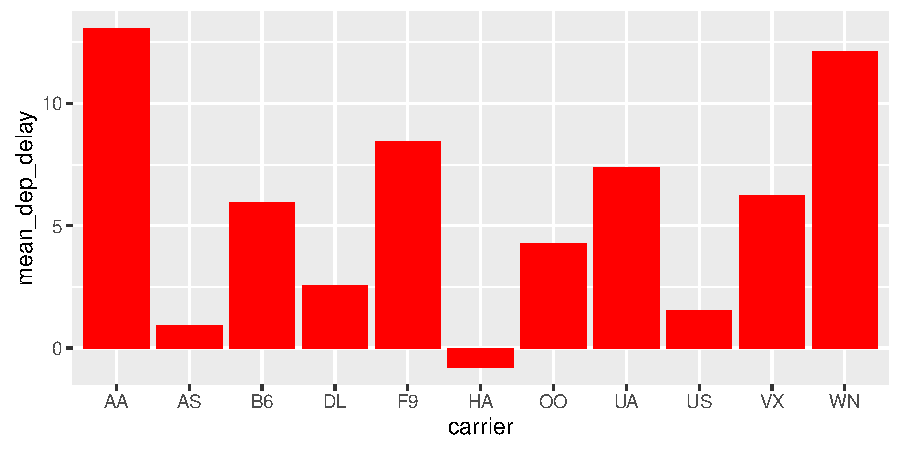
\includegraphics[angle = 0,scale = 1]{figure/delays.pdf}
  \caption[Mean Delays by Airline]{\normalsize{Mean Delays by Airline}}
  \label{fig:delays}
  \end{figure}
  
  A table linking these carrier codes to airline names is available at
  \url{https://github.com/ismayc/pnwflights14/blob/master/data/airlines.csv}.
  
  \clearpage
  
  Next, we will explore the use of the \texttt{scale} parameter which can
  be used to shrink or expand an image. Here we use the mathematical graph
  stored in the ``subdivision.pdf'' file. Note that we didn't specify the
  \texttt{caption\ =} or \texttt{label\ =} here, but we could have.
  
  \begin{Shaded}
  \begin{Highlighting}[]
  \KeywordTok{label}\NormalTok{(}\StringTok{"figure/subdivision.pdf"}\NormalTok{, }\StringTok{"Subdiv. graph"}\NormalTok{, }\StringTok{"subd"}\NormalTok{, }
        \DataTypeTok{scale =} \FloatTok{0.75}\NormalTok{)}
  \end{Highlighting}
  \end{Shaded}
  
  \begin{figure}[h!tbp]
  \centering
  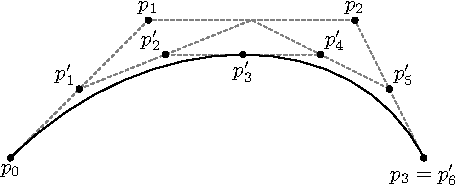
\includegraphics[angle = 0,scale = 0.75]{figure/subdivision.pdf}
  \caption[Subdiv. graph]{\normalsize{Subdiv. graph}}
  \label{fig:subd}
  \end{figure}
  
  Here is a reference to this image: \autoref{fig:subd}. (Move this around
  throughout the document as you wish.)
  
  \subsubsection{More Figure Stuff}\label{more-figure-stuff}
  
  Lastly, we will explore how to rotate figures using the \texttt{angle}
  parameter.
  
  \begin{Shaded}
  \begin{Highlighting}[]
  \KeywordTok{label}\NormalTok{(}\StringTok{"figure/subdivision.pdf"}\NormalTok{, }
        \StringTok{"A Larger Figure, Flipped Upside Down"}\NormalTok{, }
        \DataTypeTok{scale =} \FloatTok{1.5}\NormalTok{,}
        \DataTypeTok{angle =} \DecValTok{180}\NormalTok{,}
        \DataTypeTok{label =} \StringTok{"subd2"}\NormalTok{)}
  \end{Highlighting}
  \end{Shaded}
  
  \begin{figure}[h!tbp]
  \centering
  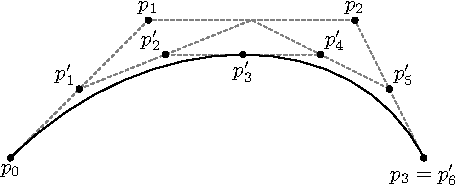
\includegraphics[angle = 180,scale = 1.5]{figure/subdivision.pdf}
  \caption[A Larger Figure, Flipped Upside Down]{\normalsize{A Larger Figure, Flipped Upside Down}}
  \label{fig:subd2}
  \end{figure}
  
  As another example, here is a reference to this figure:
  \autoref{fig:subd2}.
  
  \subsubsection{Common Modifications}\label{common-modifications}
  
  The following figure features the more popular changes thesis students
  want to make to their figures. We can add math to the caption that
  displays below the picture, specify the size of our caption to display
  below the figure (list of sizes available at this
  \href{http://www.emerson.emory.edu/services/latex/latex_169.html\#SEC169}{link}),
  and also specify that a different caption \texttt{alt.cap} be what
  appears in the Table of Figures for this figure.
  
  If you'd like to make further tweaks to figures, you might need to
  invoke some \LaTeX~code. Please email us at
  \href{mailto:data@reed.edu}{\nolinkurl{data@reed.edu}} if you need
  assistance.
  
  \begin{Shaded}
  \begin{Highlighting}[]
  \KeywordTok{label}\NormalTok{(}\StringTok{"figure/subdivision.pdf"}\NormalTok{, }
        \DataTypeTok{caption =} \StringTok{"Subdivision of arc segments"}\NormalTok{,}
        \DataTypeTok{alt.cap =} \StringTok{"You can see that $p_3 = p_6^}\CharTok{\textbackslash{}\textbackslash{}}\StringTok{prime$"}\NormalTok{,}
        \DataTypeTok{cap.size =} \StringTok{"footnotesize"}\NormalTok{,}
        \DataTypeTok{label =} \StringTok{"subd3"}\NormalTok{)}
  \end{Highlighting}
  \end{Shaded}
  
  \begin{figure}[h!tbp]
  \centering
  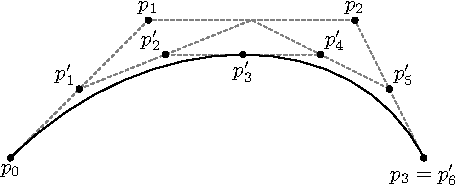
\includegraphics[angle = 0,scale = 1]{figure/subdivision.pdf}
  \caption[Subdivision of arc segments]{\footnotesize{You can see that $p_3 = p_6^\prime$}}
  \label{fig:subd3}
  \end{figure}
  
  \section{Footnotes and Endnotes}\label{footnotes-and-endnotes}
  
  You might want to footnote something.\footnote{footnote text} The
  footnote will be in a smaller font and placed appropriately. Endnotes
  work in much the same way. More information can be found about both on
  the CUS site or feel free to reach out to
  \href{mailto:data@reed.edu}{\nolinkurl{data@reed.edu}}.
  
  \section{Bibliographies}\label{bibliographies}
  
  Of course you will need to cite things, and you will probably accumulate
  an armful of sources. There are a variety of tools available for
  creating a bibliography database (stored with the .bib extension). In
  addition to BibTeX suggested below, you may want to consider using the
  free and easy-to-use tool called Zotero. The Reed librarians have
  created Zotero documentation at
  \url{http://libguides.reed.edu/citation/zotero}. In addition, a tutorial
  is available from Middlebury College at
  \url{http://sites.middlebury.edu/zoteromiddlebury/}.
  
  \emph{R Markdown} uses \emph{pandoc} (\url{http://pandoc.org/}) to build
  its bibliographies. One nice caveat of this is that you won't have to do
  a second compile to load in references as standard \LaTeX~requires. To
  cite references in your thesis (after creating your bibliography
  database), place the reference name inside square brackets and precede
  it by the ``at'' symbol. For example, here's a reference to a book about
  worrying: (Molina \& Borkovec, 1994). This \texttt{Molina1994} entry
  appears in a file called \texttt{thesis.bib} in the \texttt{bib} folder.
  This bibliography database file was created by a program called BibTeX.
  You can call this file something else if you like (look at the YAML
  header in the main .Rmd file) and, by default, is to placed in the
  \texttt{bib} folder.
  
  For more information about BibTeX and bibliographies, see our CUS site
  (\url{http://web.reed.edu/cis/help/latex/index.html})\footnote{Reed~College
    (2007)}. There are three pages on this topic: \emph{bibtex} (which
  talks about using BibTeX, at
  \url{http://web.reed.edu/cis/help/latex/bibtex.html}),
  \emph{bibtexstyles} (about how to find and use the bibliography style
  that best suits your needs, at
  \url{http://web.reed.edu/cis/help/latex/bibtexstyles.html}) and
  \emph{bibman} (which covers how to make and maintain a bibliography by
  hand, without BibTeX, at
  \url{http://web.reed.edu/cis/help/latex/bibman.html}). The last page
  will not be useful unless you have only a few sources.
  
  If you look at the YAML header at the top of the main .Rmd file you can
  see that we can specify the style of the bibliography by referencing the
  appropriate csl file. You can download a variety of different style
  files at \url{https://www.zotero.org/styles}. Make sure to download the
  file into the csl folder.
  
  \paragraph{Tips for Bibliographies}\label{tips-for-bibliographies}
  
  \begin{itemize}
  \tightlist
  \item
    Like with thesis formatting, the sooner you start compiling your
    bibliography for something as large as thesis, the better. Typing in
    source after source is mind-numbing enough; do you really want to do
    it for hours on end in late April? Think of it as procrastination.
  \item
    The cite key (a citation's label) needs to be unique from the other
    entries.
  \item
    When you have more than one author or editor, you need to separate
    each author's name by the word ``and'' e.g.
    \texttt{Author\ =\ \{Noble,\ Sam\ and\ Youngberg,\ Jessica\},}.
  \item
    Bibliographies made using BibTeX (whether manually or using a manager)
    accept \LaTeX~markup, so you can italicize and add symbols as
    necessary.
  \item
    To force capitalization in an article title or where all lowercase is
    generally used, bracket the capital letter in curly braces.
  \item
    You can add a Reed Thesis citation\footnote{Noble (2002)} option. The
    best way to do this is to use the phdthesis type of citation, and use
    the optional ``type'' field to enter ``Reed thesis'' or
    ``Undergraduate thesis.''
  \end{itemize}
  
  \section{Anything else?}\label{anything-else}
  
  If you'd like to see examples of other things in this template, please
  contact the Data @ Reed team (email
  \href{mailto:data@reed.edu}{\nolinkurl{data@reed.edu}}) with your
  suggestions. We love to see people using \emph{R Markdown} for their
  theses, and are happy to help.
  
  \chapter*{Conclusion}\label{conclusion}
  \addcontentsline{toc}{chapter}{Conclusion}
  
  \setcounter{chapter}{4} \setcounter{section}{0}
  
  If we don't want Conclusion to have a chapter number next to it, we can
  add the \texttt{\{.unnumbered\}} attribute. This has an unintended
  consequence of the sections being labeled as 3.6 for example though
  instead of 4.1. The \LaTeX~commands immediately following the Conclusion
  declaration get things back on track.
  
  \subsubsection{More info}\label{more-info}
  
  And here's some other random info: the first paragraph after a chapter
  title or section head \emph{shouldn't be} indented, because indents are
  to tell the reader that you're starting a new paragraph. Since that's
  obvious after a chapter or section title, proper typesetting doesn't add
  an indent there.
  
  \appendix
  
  \chapter{The First Appendix}\label{the-first-appendix}
  
  This first appendix includes all of the R chunks of code that were
  hidden throughout the document (using the \texttt{include\ =\ FALSE}
  chunk tag) to help with readibility and/or setup.
  
  \subsubsection{In the main Rmd file:}\label{in-the-main-rmd-file}
  
  \begin{Shaded}
  \begin{Highlighting}[]
  \CommentTok{# This chunk ensures that the reedtemplates package is}
  \CommentTok{# installed and loaded. This reedtemplates package includes}
  \CommentTok{# the template files for the thesis and also two functions}
  \CommentTok{# used for labeling and referencing}
  \NormalTok{if(!}\KeywordTok{require}\NormalTok{(devtools))}
    \KeywordTok{install.packages}\NormalTok{(}\StringTok{"devtools"}\NormalTok{, }\DataTypeTok{repos =} \StringTok{"http://cran.rstudio.com"}\NormalTok{)}
  \NormalTok{if(!}\KeywordTok{require}\NormalTok{(reedtemplates))\{}
    \KeywordTok{library}\NormalTok{(devtools)}
    \NormalTok{devtools::}\KeywordTok{install_github}\NormalTok{(}\StringTok{"ismayc/reedtemplates"}\NormalTok{)}
  \NormalTok{\}}
  \KeywordTok{library}\NormalTok{(reedtemplates)}
  \end{Highlighting}
  \end{Shaded}
  
  \subsubsection{\texorpdfstring{In
  \protect\hyperlink{ref_labels}{}:}{In :}}\label{in}
  
  \begin{Shaded}
  \begin{Highlighting}[]
  \CommentTok{# This chunk ensures that the reedtemplates package is}
  \CommentTok{# installed and loaded. This reedtemplates package includes}
  \CommentTok{# the template files for the thesis and also two functions}
  \CommentTok{# used for labeling and referencing}
  \NormalTok{if(!}\KeywordTok{require}\NormalTok{(devtools))}
    \KeywordTok{install.packages}\NormalTok{(}\StringTok{"devtools"}\NormalTok{, }\DataTypeTok{repos =} \StringTok{"http://cran.rstudio.com"}\NormalTok{)}
  \NormalTok{if(!}\KeywordTok{require}\NormalTok{(dplyr))}
      \KeywordTok{install.packages}\NormalTok{(}\StringTok{"dplyr"}\NormalTok{, }\DataTypeTok{repos =} \StringTok{"http://cran.rstudio.com"}\NormalTok{)}
  \NormalTok{if(!}\KeywordTok{require}\NormalTok{(ggplot2))}
      \KeywordTok{install.packages}\NormalTok{(}\StringTok{"ggplot2"}\NormalTok{, }\DataTypeTok{repos =} \StringTok{"http://cran.rstudio.com"}\NormalTok{)}
  \NormalTok{if(!}\KeywordTok{require}\NormalTok{(reedtemplates))\{}
    \KeywordTok{library}\NormalTok{(devtools)}
    \NormalTok{devtools::}\KeywordTok{install_github}\NormalTok{(}\StringTok{"ismayc/reedtemplates"}\NormalTok{)}
    \NormalTok{\}}
  \KeywordTok{library}\NormalTok{(reedtemplates)}
  \CommentTok{#flights <- read.csv("data/flights.csv")}
  \end{Highlighting}
  \end{Shaded}
  
  \chapter{The Second Appendix, for
  Fun}\label{the-second-appendix-for-fun}
  
  \backmatter
  
  \chapter{References}\label{references}
  
  \noindent
  
  \setlength{\parindent}{-0.20in} \setlength{\leftskip}{0.20in}
  \setlength{\parskip}{8pt}
  
  \hypertarget{refs}{}
  \hypertarget{ref-angel2000}{}
  Angel, E. (2000). \emph{Interactive computer graphics : A top-down
  approach with opengl}. Boston, MA: Addison Wesley Longman.
  
  \hypertarget{ref-angel2001}{}
  Angel, E. (2001a). \emph{Batch-file computer graphics : A bottom-up
  approach with quicktime}. Boston, MA: Wesley Addison Longman.
  
  \hypertarget{ref-angel2002a}{}
  Angel, E. (2001b). \emph{Test second book by angel}. Boston, MA: Wesley
  Addison Longman.
  
  \hypertarget{ref-Molina1994}{}
  Molina, S. T., \& Borkovec, T. D. (1994). The Penn State worry
  questionnaire: Psychometric properties and associated characteristics.
  In G. C. L. Davey \& F. Tallis (Eds.), \emph{Worrying: Perspectives on
  theory, assessment and treatment} (pp. 265--283). New York: Wiley.
  
  \hypertarget{ref-noble2002}{}
  Noble, S. G. (2002). \emph{Turning images into simple line-art}
  (Undergraduate thesis). Reed College.
  
  \hypertarget{ref-reedweb2007}{}
  Reed~College. (2007, march). LaTeX your document. Retrieved from
  \url{http://web.reed.edu/cis/help/LaTeX/index.html}


  % Index?

\end{document}

